\documentclass[11pt,a4paper]{article}
\usepackage{amsmath,amssymb,amsfonts,url}
\usepackage{xcolor}
\usepackage[margin=2cm]{geometry}
\usepackage[T1]{fontenc}
\usepackage{ pifont}
\usepackage{multicol}
\usepackage{ulem}
\usepackage{todonotes}   %[disable] option
\allowdisplaybreaks

\renewcommand{\rmdefault}{phv}

\usepackage{pgfgantt}
\newcommand\textganttbar[4]{%
    \ganttbar{#1}{#3}{#4}
    \ganttbar[inline]{#2}{#3}{#4}
}

% ----------------------------------------------------------------
\vfuzz2pt % Don't report over-full v-boxes if over-edge is small
\hfuzz2pt % Don't report over-full h-boxes if over-edge is small

% Hilary's addition to make a compact article and use latex section commands
% make list and enumerate more compact
\usepackage{tweaklist}
\renewcommand{\itemhook}
{
    \setlength{\topsep}{3pt}
    \setlength{\parskip}{0pt}
    \setlength{\parsep}{0pt}
    \setlength{\partopsep}{0pt}
    \setlength{\itemsep}{0pt}
    \setlength{\labelwidth}{10pt}
    \setlength{\leftmargin}{\labelwidth}
}

\renewcommand{\enumhook}
{
    \setlength{\topsep}{3pt}
    \setlength{\parskip}{0pt}
    \setlength{\parsep}{0pt}
    \setlength{\partopsep}{0pt}
    \setlength{\itemsep}{3pt}
    \setlength{\labelwidth}{10pt}
    \setlength{\leftmargin}{\labelwidth}
}

\renewcommand{\deschook}
{
    \setlength{\topsep}{3pt}
    \setlength{\parskip}{0pt}
    \setlength{\parsep}{0pt}
    \setlength{\partopsep}{0pt}
    \setlength{\itemsep}{0pt}
    \setlength{\labelwidth}{0pt}
    \setlength{\leftmargin}{\labelwidth}
}

% Compact sections and parts
\makeatletter
\def\@part[#1]#2
{%
    \refstepcounter{part}%
    {%
        \parindent \z@ \raggedright \interlinepenalty \@M
        \normalfont \Large\bfseries\raggedright
        \partname\nobreakspace\thepart : \nobreakspace #2 %\markboth{}{}\par
    }%
    \nobreak \vskip 1.3ex \@afterheading%
}
\renewcommand\section
{%
    \@startsection {section}{1}{\z@}{-1ex \@plus -0.5ex \@minus -.1ex}%
   {0.5ex \@plus.1ex}{\large\bfseries\raggedright}%
}
\renewcommand\subsection%
{%
    \@startsection {subsection}{1}{\z@}{-1ex \@plus -0.5ex \@minus-.1ex}%
   {0.5ex \@plus .1ex}{\normalfont\bfseries\raggedright}%
}
\renewcommand\subsubsection%
{%
    \@startsection {subsubsection}{1}{\z@}{-0.5ex \@plus -1ex \@minus -.2ex}%
   {0.1ex \@plus .1ex}{\normalfont\bfseries\raggedright}%
}
\renewcommand\paragraph{\@startsection{paragraph}{4}{\z@}%
                                    {0.5ex \@plus0.5ex \@minus.1ex}%
                                    {-0.5em}%
                                    {\normalfont\normalsize\bfseries}}

% subsubsections are actually work packages
\renewcommand{\thesubsubsection}{WP\arabic{subsubsection}}% \hspace{-1em}}
\newcommand\workPackage{\@startsection{subsubsection}{3}{\z@}%
                       {-1ex \@plus -0.5ex \@minus -.1ex}%
                       {0.5ex \@plus .1ex}{\normalfont\bf\raggedright}}

\setcounter{secnumdepth}{5}

% paragraphs are sub work packages
\renewcommand{\theparagraph}{WP\arabic{subsubsection}\alph{paragraph}}%
\newcommand\subworkPackage{\@startsection{paragraph}{4}{\z@}%
                                    {0.5ex \@plus0.5ex \@minus.1ex}%
                                    {-0.5em}%
                                    {\normalfont\normalsize\bfseries}}

\def\@maketitle
{%
  \begin{center}%
  \let \footnote \thanks
    {\large\bf \@title \par}%
    \vskip 0.5em%
    {\normalfont
      \lineskip 1em%
      \begin{tabular}[t]{c}%
        \@author
      \end{tabular}\par}%
    \vskip 0.5em%
    {\large \@date}%
  \end{center}%
  \vskip -2.5em
  \par
  \vskip -1.5em
}
% Reduce the spacing around equations
\AtBeginDocument{%
 \abovedisplayskip=6pt plus 6pt minus 4pt
 \belowdisplayskip=6pt plus 6pt minus 3pt
 \abovedisplayshortskip=0pt plus 3pt
 \belowdisplayshortskip=7pt plus 3pt minus 4pt
}
\setlength{\jot}{0pt}% Inter-equation spacing
\makeatother

% Bibliography stuff
%\usepackage[square,sort&compress,numbers,super]{natbib}
\usepackage[round,sort&compress]{natbib}
%\usepackage[style=authoryear,citetracker,backref, backend=biber]{biblatex}

\setlength{\bibsep}{0pt}
\setlength{\bibhang}{6pt}

% modification to natbib to remove margin
\makeatletter
\renewcommand\NAT@bibsetnum[1]{\settowidth\labelwidth{\@biblabel{#1}}%
%   \setlength{\leftmargin}{\labelwidth}\addtolength{\leftmargin}{\labelsep}%
   \setlength{\leftmargin}{0pt}\addtolength{\leftmargin}{0pt}%
   \setlength{\itemsep}{\bibsep}\setlength{\parsep}{\z@}%
   \setlength{\itemindent}{\bibindent}%
   \ifNAT@openbib
     \addtolength{\leftmargin}{\bibindent}%
     \setlength{\itemindent}{-\bibindent}%
     \setlength{\listparindent}{\itemindent}%
     \setlength{\parsep}{0pt}%
   \fi
}
\makeatother


\begin{document}

\title{Case For Support \\ \Large
Multi-fluid modelling of convection
}
\author{Hilary Weller \and Georgios Efstathiou \and John Thuburn \and William McIntyre \and Daniel Shipley}
\date{}
\maketitle

\part{Track Record}

% JT
The proposed project will require interdisciplinary expertise in atmospheric physics and fluid dynamics
and in the development of improved numerics and physical parameterisations for atmospheric models.
We have assembled a research team that has the necessary breadth and depth of expertise and is built on
existing strong collaborations.

%{\color{red} I've shortened the section on JT a bit, but we'll need more trimming to fit in Dan and Will.}

\paragraph*{Dr Hilary Weller (Reading)} holds a faculty position in Meteorology at Reading. She has been the lead PI on three NERC grants on atmospheric modelling. Working as a PI on the Met Office/NERC/STFC ``Gung-Ho'' project, Hilary collaborated with Met Office staff creating and analysing long time step transport schemes \cite[]{CWPS17,SWMD17} and finding optimal coupling between fast and slow processes \cite[][]{WLW13}. She led pioneering work analysing numerical methods for quasi-uniform grids of the sphere \cite[e.g.][]{Wel12,WTC12} and proposed improvements in modelling flow over orography \cite[]{WS14}. 

Before numerical modelling, Dr Weller worked on tropical meteorology \cite[e.g.][]{LGWS09}. These have been combined, proposing, with Prof. Thuburn, the use of multi-fluid modelling for representing sub-grid-scale convection \cite[]{TWV+18} and creating the first numerical method to solve these equations \cite[]{WM19} as a Co-I on the NERC/Met Office Paracon projects to improve the modelling of convection in atmospheric models.

\paragraph*{Dr Georgios Efstathiou (Exeter)} is a NERC Independent Research Fellow working on grey-zone turbulence modelling. He has over 15 years of experience in research on the modelling of
atmospheric processes at various scales, from turbulent motions in the boundary layer
to heavy precipitation synoptic systems. An overarching theme is understanding the
connections between atmospheric scales with the aim to improve high-resolution
numerical weather prediction. He has conducted many Large Eddy Simulation (LES) studies and used LES to identify 
the characteristics of the boundary-layer grey zone \citep[e.g.][]{efstathiou2015}
and develop parameterisations suitable for sub-kilometre, very high-resolution models 
\citep{efstathiou2016}. One of his main contributions in grey zone 
studies was the extension of dynamic sub-grid models from the LES to the grey zone region 
providing adaptive and scale dependent turbulence length scales for sub-grid models 
\citep{efstathiou2018,efstathiou2019a}. As part of the NERC/Met Office ParaCon 
project he has developed a novel method to identify updrafts in convective flows 
by optimising the multi-fluid decomposition of the atmosphere \citep{ETB20}.

\paragraph*{Prof. John Thuburn (Exeter)} holds a Chair in Geophysical Fluid Dynamics at the University of Exeter, jointly
funded by the Met Office under the Met Office Academic Partnership.
Since 2000 he has collaborated closely with the Met Office on numerical methods for their
weather and climate models. He made important contributions to the development of the
ENDGame dynamical core \cite[e.g.][]{WSW+14}, which is now a major operational success.
% Could drop the next two sentences
Since 2011 he has collaborated with the Met Office and other UK academic partners on the ``Gung-Ho''
project to develop a future dynamical core suitable for massively parallel computer
architectures, \citep[e.g.][]{MBS+19}.
%An important theme is to capture key aspects of accuracy related to balance and
%conservation on non-traditional grids \cite[e.g.][]{TC15}.
%The coupling of physical parameterisations and sub-grid models to resolved dynamics is often
%particularly subtle because the coupling occurs via marginally resolved and imperfectly
%represented scales.
%Prof.\ Thuburn has contributed to understanding these numerical aspects
%of physics-dynamics coupling in the context of quasi-two-dimensional turbulent cascades \cite[e.g.][]{TKW14} and %boundary layer parameterisations \cite[]{HTW13a}.
He has contributed to the emerging field of physics-dynamics coupling for atmospheric models.
Most relevant for the present proposal is that,
together with co-authors, he developed the mathematical framework for the multi-fluid
approach \citep[][]{TWV+18}, analysed the conservation and normal mode properties
of the unparameterised multi-fluid equations \citep[][]{TV18}, and demonstrated
a proof of concept for a single-column model of the dry convective boundary-layer \citep[][]{TEB19}.

\todo[inline]{Please edit}
\paragraph*{Dr William McIntyre} has been a PDRA on the Paracon project at Exeter since October 2020 where he has been working on multi-fluid modelling of convection and is writing up a paper on single-column modelling of moist convection. Will was awarded his PhD from Reading in October 2020 on ``Multi-fluid modelling of dry convection''. His work on numerical methods will enable some of the outcomes of this project \cite{MWH20}. Will won the poster prize in 2019 ... and subsequently gave an invited talk at a Royal ...

\todo[inline]{Please edit}
\paragraph*{Mr Daniel Shipley} is a PhD student at Reading supervised by Hilary Weller and Prof Peter Clark and is due to submit in xxx 2021. He is writing up papers on theoretical aspects of multi-fluid modelling and on multi-fluid modelling of Rayleigh-B\'{e}nard convection. Dan's theoretical work will lay the groundwork for this project. Dan also won the poster prize in 202x ...

\section*{Institutions}

\paragraph*{The University of Reading Meteorology department} is one of the largest of its kind in Europe with 50 academic staff, 20 senior research staff and fellowship holders, around 90 postdocs and around 70 PhD students. In the 2014 Research Excellence Framework (REF), 86\% of their research was graded as world leading or internationally excellent. Their ``research power'' places them 3rd in the country in Earth Systems and Environmental Science, and the impact of their research was rated 9th highest in the country. The University is a formal Academic Partner of the Met Office and hosts about 20 Met Office scientists. The Reading PDRA will attend Mesoscale Meteorology Group meetings and weekly seminars on atmosphere and ocean science.

\paragraph*{The Department of Mathematics at the University of Exeter} includes the Geophysical and Astrophysical Fluid Dynamics and Exeter Climate Systems research groups, who between them have over~50 staff and over~40 PhD students researching topics related to weather, climate, and modelling. Both groups have excellent track records of collaboration with the Met Office. In the 2014 REF, for UoA 10 (Mathematical Sciences) 83\% of their research was assessed as world leading (4*) or internationally excellent (3*), while for UoA~7 (Earth Systems and Environmental Sciences) 89\% of their research was assessed as 4* or 3*.

\paragraph*{The Met Office} is a world leader in weather forecasting and climate prediction, and their atmospheric model is used by many operational centres (for example, the Australian Bureau of Meteorology). The convection parameterisation group, led by Dr Alison Stirling, publishes widely about their research on aspects of convection, weather prediction and parameterisation. They have just developed a new flexible convection scheme called CoMorph, which will be the basis for future convection developments at the Met Office. Alison's group contributes to ensuring that the Met Office model maintains its high skill and the Met Office maintains its international reputation in numerical weather prediction, climate projection and research. 

\input{trackRecord.bbl}

\newpage

\part{Research Proposal}

\section{Motivation and Summary}

The representation of sub-grid-scale convection is arguably the weakest aspect of current weather and climate models, leading to unrealistic simulations of monsoons, the diurnal cycle of rainfall, the Madden-Julian Oscillation, and convectively coupled waves  \cite[]{SAB+13,HPB+14}. The representation of the sub-grid-scale flow becomes particularly challenging at resolutions where convection is partially resolved -- the grey zone -- as assumptions behind current parameterisations, such as local subsidence, are grossly violated \cite[e.g.][]{GG05}.

The problem is so bad that weather forecast models are run without convection parameterisation as soon as the resolution is high enough to partially resolve convection, even though there is plenty of sub-grid-scale convection that should be parameterised if only the schemes did not introduce large errors \cite[]{LCD+08}. The same problems occurs with climate models and vast computers are used to increase resolution so that convection paramterisation can be avoided even though there still should be some sub-grid-scale convection \cite[]{SSJ+19}. We aim to improve the modelling of convection to enable more accurate simulations at coarse resolution and to accurately represent sub-grid-scale convection when convection is partially resolved. 

Standard convection schemes are based on a simplified representation of vertical fluxes in terms of a division of the sub-grid flow into separate, homogeneous flows such as updraft, downdraft and environment, with assumptions of small updraft area fraction and horizontally homogeneous quasi-equilbrium, implying no net mass flux (local subsidence) and no horizontal transports or propagation. The multi-fluid approach removes these assumptions and has shown promise in single-column models. However it is as yet unproven in three-dimensional models and does not address sub-grid variability beyond the multi-fluid division. High-order (or multi-moment) turbulence modelling predicts moments of probability distributions of sub-grid variability. The multi-fluid and multi-moment approaches thus provide two different ways of accounting for sub-grid variability in models, each likely to be most useful in different regimes. Their unification has the potential to work well across a much wider range of regimes, in particular, enabling the construction of a scale-aware model that is applicable at a range of resolutions encompassing the grey zones.

Our overarching aim is to advance the fundamental physics based understanding of turbulent convection in order to develop a three-dimensional, multi-fluid, multi-moment model with a seamless transition from fully sub-grid, through the grey zone and to resolved convection. We will proceed incrementally, building on existing models and developing improved or completely new parameterisations, gradually adding complexity to the model formulation and to the test cases simulated.
A multi-fluid model with a simplified multi-moment representation has already been shown to work well in a single column, so we will start by simulating fully sub-grid convection in three dimensions using similar parameterisations.
There is scope to improve these parameterisations which will be needed to simulate partially resolved convection. 
To formulate these improvements we will use a variety of approaches, all ultimately founded on comprehensive diagnostics of high-resolution LES data to provide a `ground truth'.
%{\color{red} NEEDS WORK To formulate these improved parameterisations, complete multi-fluid and multi-moment budgets will be diagnosed from high resolution LES and combined with a toolbox of methods.}
The new approach will be evaluated using a suite of equilibrium and non-equilibrium test cases of convective growth and propagation. A key deliverable will be an open source community model enabling the future research needed to develop the approach towards operational use.

%We will explore the sensitivity of the accuracy to the number of fluids versus the number of moments that are used and which moments should be diagnostic or prognostic (i.e. which level of the Mellor-Yamada hierarchy). We will need to find an appropriate turbulence length scale in a multi-fluid context.

%This proposal will describe a toolbox of methods for finding new closures. High resolution LES will be used to diagnose multi-fluid and multi-moment budgets and evaluate closures. 


\section{Scientific Background}

Coarse resolution models must represent the effects of sub-grid-scale convection, otherwise convection is forced to occur at the model grid scale resulting in highly unrealistic behaviour and possibly model instability \cite[]{PY15}.
As supercomputers increase in power, convection can be better resolved over larger areas \cite[e.g.][]{GC17}, but fully resolved convection is not likely to be achieved in the foreseeable future for global weather prediction or routine climate modelling \cite[e.g.][]{SSJ+19}; thus, there is an ongoing need to represent the effects of sub-grid-scale convection.
Typical operational convection schemes are built on a set of simplifying approximations:
heat, moisture and momentum are re-distributed in the vertical, but not mass \cite[implying local subsidence,][]{Tied89,GR90}; convection is assumed to be in equilibrium with the large scale so limited account is taken of convective memory and the gradual build up of convection; convection in one grid column is assumed to be independent of its neighbours and advection of convective systems is neglected. These simplifying approximations are believed to limit the accuracy and physical fidelity of
convection in weather and climate models. Despite recent valuable improvements, such as relaxing the quasi-equilibrium assumption \cite[]{PR98,GG05,Par14} and adding stochasticity \cite[]{PC08}, it has not been possible to develop schemes that work well when convection is partially resolved.

\cite{TWV+18} proposed a new approach --- multi-fluid modelling of convection --- in which convective updrafts, downdrafts and the stable environment are modelled as distinct fluids with separate, but consistent, momentum, continuity, energy and moisture transport equations. The fluids interact via entrainment, detrainment and pressure terms. 
The leading order dynamics of convection, including non-equilibrium effects, net mass transport, and other horizontal and vertical transports, is explicitly described by these equations, allowing them to be represented by
an extended numerical model dynamical core. Although some processes must still be parameterised, including entrainment,
detrainment, and small scale turbulent fluxes, these are far fewer than with a traditional convection scheme.
The multi-fluid approach has similarities with the extended Eddy-Diffusivity Mass-Flux (EDMF) scheme of \cite{TKP+18} who added time derivatives to the EDMF equations.

Mass flux convection schemes focus on representing the transport due to sub-grid-scale coherent structures such as
updrafts. An alternative approach to representing sub-grid-scale transports is to solve prognostic or diagnostic
equations for a range of second-order moments. This multi-moment approach is most commonly used for the
boundary layer, and is exemplified by the \citet{mellor1973,mellor1974,mellor1982} MY hierarchy of turbulence
closure models.
There are several reasons for expecting a unification of the multi-fluid and multi-moment approaches to enable
significant advances. It would avoid an artificial separation of boundary layer and convection schemes.
It would enable multi-moment information to be used in the multi-fluid parameterised terms, particularly
entrainment and detrainment. It would enable a more physically based parameterisation of sub-grid turbulent
fluxes, including, for example, up gradient fluxes such as those due to the fallback of thermals
overshooting the boundary layer inversion. Most importantly, it would provide a framework
with the potential to work smoothly across the grey zone from fully resolved to fully sub-grid convection.

\todo[inline]{The following 2 paragraphs are great but I think are out of place in this scientific background section. The same material is covered in the summary, relationship with Paracon and the proposed research. Can they be dropped or incorporated into the summary?}
We have derived the governing equations for the multi-fluid analogue of the MY hierarchy, but there remain
some key questions, which we aim to investigate. Which combination of multiple fluids and multiple moments
most efficiently describes the sub-grid processes, and does the answer depend on flow regime or model resolution?
How can multi-moment information be best used to inform multi-fluid entrainment and detrainment terms?
How must tuneable coefficients in the MY system, e.g.\ in defining  the unresolved turbulent length scales, be modified
for the multi-fluid case and what is their resolution dependence across the scales (e.g. in the grey zone)?

Existing parameterisations of entrainment and detainment, and eddy diffusive representation of small scale turbulent
fluxes, will provide a valuable starting point for the proposed work, and we have had some success with them in
single column models. However, further work is needed to adapt these parameterisations for three-dimensional models,
and especially to formulate the grid-scale dependence that will enable them to work seamlessly across the grey zone.
Discovering quantitatively and causally correct parameterisations is difficult when processes are complex, as in moist
convection. Our approach will be to build upon existing parameterisations, incorporating physical and fluid dynamical
understanding, and extending them, for example, using Assumed PDFs (APDFs) and the theory of distributions, incorporating
multi-moment information where appropriate. Important physical and mathematical constraints on the formulation will
be taken into account. Vital to this work will be detailed diagnostics of LES data to validate proposed formulations
and to motivate new ones.

\section{Outline Formulation of Multi-fluid Modelling of Convection}
\label{sec:mf}

To provide more background to the proposed research we present here the
multi-fluid, dry Boussinesq Navier-Stokes equations \cite[approximated by][]{WMS20} (though the model to be developed will, in fact,
use an anelastic approximation):
\begin{eqnarray}
\frac{\partial\sigma_{i}}{\partial t}+\nabla\cdot(\sigma_{i}\mathbf{u}_{i}) & = & {\textstyle\sum}_{j\ne i}\left\{ M_{ji}-M{}_{ij}\right\} ,\label{eq:sigma}\\
\frac{D_{i}\mathbf{u}_{i}}{Dt}+\nabla P_{i} & = & b_{i}\mathbf{k}+\nabla\cdot \mathsf{T}_i +\frac{1}{\sigma_{i}}{\textstyle\sum}_{j\ne i}\left\{ M_{ji}\left(\mathbf{u}_{ji}^{T}-\mathbf{u}_{i}\right)-M_{ij}\left(\mathbf{u}_{ij}^{T}-\mathbf{u}_{i}\right)\right\} , \label{eq:mom}\\
\frac{D_{i}b_{i}}{Dt} & = & -\nabla\cdot \mathbf{F}^b_{i} +\frac{1}{\sigma_{i}}{\textstyle\sum}_{j\ne i}\left\{ M_{ji}\left(b_{ji}^{T}-b_{i}\right)-M_{ij}\left(b_{ij}^{T}-b_{i}\right)\right\} , \label{eq:b}\\
{\textstyle\sum}_{i}\nabla\cdot\sigma_{i}\mathbf{u}_{i} & = & 0 , \label{eq:divFree}\\
{\textstyle\sum}_{i}\sigma_{i} & = & 1.\label{eq:sumOne}
\end{eqnarray}
Here $\sigma_i$, $\mathbf{u}_i$, $b_i$ and $P_i$ are the volume fraction, velocity, buoyancy and pressure of fluid $i$. (The fluid pressures are different from partial pressures of gases because the fluids are not mixed or in equilibrium.) Representing moist convection also needs transport equations for moisture in each fluid and a latent heating term in the buoyancy equation. $M_{ij}$ is the mass transfer rate from fluid $i$ to $j$, representing entrainment and detrainment. $\mathbf{u}_{ij}^T$ is the mean velocity of the fluid that is transferred from $i$ to $j$ and $b_{ij}^T$ is the mean buoyancy of the fluid that is transferred. 
$\mathsf{T}_i$ is the stress tensor and $\mathbf{F}^b_{i}$ the buoyancy flux that arise because of sub-grid-scale in-homogeneity.
Additional equations are needed if we wish to diagnose or predict higher-order moments.

The multi-fluid equations can represent sub-grid-scale convection if, for example, fluid 0 is the stable environment, fluid 1 is updrafts and fluid 2 is downdrafts. There are similarities between equations (\ref{eq:sigma}-\ref{eq:b}) and some conventional non-equilibrium convection parameterisations with one-dimensional prognostic equations for plume properties \cite[e.g.][]{GG05} although even non-equilibrium schemes do not couple the parameterised convection with the dynamics correctly by solving equivalents of (\ref{eq:sigma}-\ref{eq:b})  simultaneously with (\ref{eq:divFree}) (or a compressible version of (\ref{eq:divFree})). However the fact that existing parameterisations solve similar equations implies that the cost of solving the multi-fluid equations will be similar to existing parameterisations.

For the multi-fluid equations to represent sub-grid-scale convection, several terms in (\ref{eq:sigma}-\ref{eq:sumOne}) must be parameterised:
\begin{itemize}
\item rates of mass transfer between fluids, $M_{ij}$, to represent entrainment and detrainment;
\item the properties of the transferred fluid, buoyancy $b_{ij}^T$, moisture $q_{ij}^T$, and momentum $\mathbf{u}_{ij}^T$; 
\item pressure differences between fluids (the mean pressure is determined by incompressibility \eqref{eq:divFree});
\item sub-grid-scale fluxes for each fluid, $\mathsf{T}_i$, $\mathbf{F}^b_{i}$, and the corresponding moisture fluxes $\mathbf{F}^q_{i}$.
\end{itemize}

As a starting point, sub-grid-scale fluxes can be parameterised as down gradient diffusion with simple formulations for the turbulent diffusivities,
while the properties of transferred fluid can be modelled in terms of the mean properties of fluids~$i$ and~$j$. 
However, we have found improved results in our single-column model by allowing the turbulent diffusivities to depend upon predicted turbulent
kinetic energies, and by allowing the properties of transferred fluid to depend upon estimates of the sub-grid variances of moisture and vertical velocity.
These results motivate us to pursue the development of a more complete multi-moment, multi-fluid model.

\section{Relationship with ParaCon and building on our Track Record}

The poor state of convection parameterisation was the motivation for the \pounds 10M joint NERC, Met Office ParaCon project, which aims to make a ``step change in our ability to predict weather and climate impacts'' by improving parameterisation suitable for existing dynamical cores. The proposed project will utilise and advance some ParaCon outcomes:
\begin{enumerate}
\item The flexible convection parameterisation scheme CoMorph has been developed for use with the Met Office Unified Model (UM). CoMorph includes new closures for entrainment and detrainment.

\item The MONC LES model was developed and used to produce simulations of convection archetypes. Simulations of the dry and moist convective boundary layer, BOMEX shallow cumuli over the tropical ocean \cite[]{HR73}, radiative-convective equilibrium (RCE), diurnal cycles of deep convection, the shallow cumulus ARM case \cite[]{BCC+02} and the transition from shallow to deep LBA case \cite[]{BFGB02} are available at multiple resolutions.

\item A method of partitioning the atmosphere into coherent thermal structures and their environment was developed \cite[]{ETB20} based on maximising the resolved transport captured by the mean fluid velocities and other properties, thereby minimising the unresolved contributions that need to be parameterised.

\item The Mellor-Yamada closures have been extended to the grey zone and implemented in the UM.

\item A moist, two-fluid, single column model was developed using a variety of entrainment/detrainment closures dependent on turbulent kinetic energy, vertical velocity convergence and atmospheric instability. The model is able to reproduce many features of the ARM case \cite[]{BCC+02}, including updraft area fraction ($\sigma_1$)  and cloud properties (Fig \ref{fig:clouds}). 

\begin{figure}
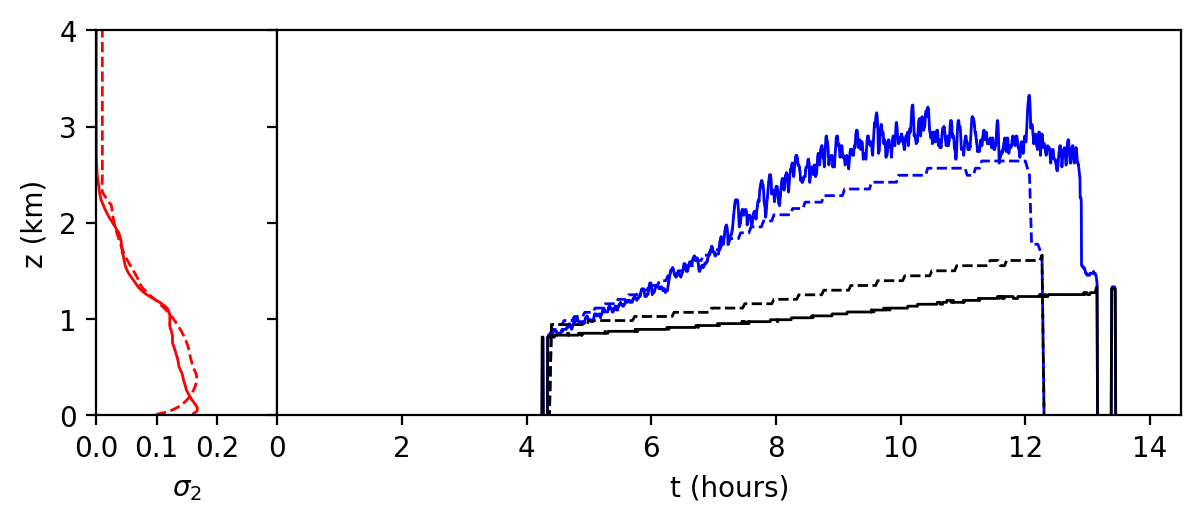
\includegraphics[width=\linewidth]{exeterScm.png}
\caption{Example results from a multi-fluid single-column model for the ARM test case. Left: the updraft fraction from the large eddy simulation (solid) and the two-fluid single-column model (dashed) at nine hours. Right: The cloud base (black) and cloud top (blue); large eddy simulation (solid) and two-fluid (dashed). A conventional parameterisation would not be able to predict this variation of $\sigma_1$ with height and this couples with the rest of the dynamics.}
\label{fig:clouds}
\end{figure}

\item A multi-fluid analogue of the Mellor-Yamada hierarchy was derived including second-moment equations for each fluid type. All of the terms in the original Mellor-Yamada formulation have analogues in the multi-fluid version. There are new terms accounting for transfers between fluids (i.e.\ entrainment and detrainment) and  terms that account for sub-grid-scale pressure fluctuations.

\item A parameterisation for pressure differences between multi-fluids based on divergence was developed and tested \cite[]{WMS20}.

\item A single column, fully compressible multi-moment, multi-fluid model with moist physics was developed at Exeter. A three-dimensional Boussinesq, dry multi-fluid model was developed at Reading based on the OpenFOAM library which will be the basis of multiFluidAtmosFOAM.

\end{enumerate}

The multi-fluid approach is not a conventional stand alone parameterisation that can be called from an existing dynamical core; in contrast to the traditional distinction between `dynamics' and parameterised `physics', it
treats the leading order dynamics of convection as part of the `dynamics'. Consequently,
it requires a bottom up redevelopment of the model formulation. For this reason, the development of the multi-fluid approach was always expected to extend beyond the end of ParaCon. In this project we will build on the progress made under ParaCon in developing both the multi-fluid approach (basic formulation, stable numerical solutions, sub-grid closures, and single column demonstrations) and the multi-moment turbulence approach by bringing them together.

\section{Proposed Research}

\subsection{Objectives}

Our overarching aim is to carry out underpinning research in turbulent convection in order to develop a three-dimensional multi-fluid model that can accurately simulate convection across a range of convection resolving to sub-grid convection resolutions.
We plan to meet this aim via the following specific objectives:

\begin{enumerate}
\item\label{it:model} Develop the software framework for a flexible, three-dimensional, multi-fluid, multi-moment model of the atmosphere including three phases of moisture. %This objective does not include finding optimal closures.

\item\label{it:budgets} Calculate comprehensive detailed diagnostics from LES data to inform the model development and for validation.

\item Develop and test suitable closures so that a single-moment, multi-fluid model simulates under resolved dry and moist convection using prescribed turbulent fluxes.

\item Implement options for prognostic and diagnostic equations for higher-order moments in the multi-fluid model. Using the approaches of section \ref{sec:tools}, optimise turbulent length scales and dissipation rates, and develop and test suitable parameterisations for coupling higher moments to transfer terms.

\item Investigate which combination of multiple fluids and multiple moments most efficiently captures sub-grid-scale
variability and transport for different types of convection and at different resolutions.

\item Evaluate using a hierarchy of convective cases from Paracon and using independent data.

\item Deliver a documented, open access, parallel, multi-fluid, multi-moment model of the atmosphere for representing convection across scales.
\end{enumerate}

\subsection{Work Packages}
\label{sec:WPs}

\workPackage{Flexible Modelling Framework (Reading, 6 months) \label{WP:model0}}

Using the OpenFOAM flexible modelling framework and building on the code developed during Paracon, we will develop multiFluidAtmosFOAM, a three-dimensional multi-fluid, multi-moment model including moisture and some simple transfer terms and closures. This will use the same anelastic approximation as the MONC LES model in order to aid comparisons. MultiFluidAtmosFOAM will use the flexible, parallel modelling framework, OpenFOAM, allowing us to focus on the equations and algorithms rather than on the spatial discretisation. This work will involve software testing and testing of exact properties such as conservation but will not aim to represent convection accurately. Combining code from Reading and Exeter will enable us to benchmark against the existing codes. All code will be version controlled and uploaded to a public \url{github.com} repository. 

\workPackage{LES Budgets (Exeter, 9 months) \label{WP:LESbudgets}}

We will compute detailed diagnostics of the LES of dry and moist convection cases produced during ParaCon, including complete budgets for all first- and second-moment quantities, pressure differences between fluids, turbulent length scales, and sub-grid PDFs, for the cases of a single fluid, two fluids (updraft and environment), and, for LBA, three fluids (updraft, downdraft, and environment).
We will decompose the flow into updrafts and their environment using the optimal decomposition developed during Paracon and extend this to diagnose coherent downdrafts. The budgets will be calculated for a range of horizontal filter scales, from a global horizontal average down to scales comparable to the cloud width and boundary layer depth.


\workPackage{Multi-fluid modelling of dry convection (Reading, 6 months) \label{WP:dryMF}}

In order to build complexity gradually, we will develop parameterisations for transfers and pressure differences between fluids for the dry convective boundary layer based on the budgets and pressure differences calculated in \ref{WP:LESbudgets} and using the methods described in section \ref{sec:tools}. In this WP, we will not attempt to predict second-moment quantities but instead use the values of second-order moments from \ref{WP:LESbudgets}, thus reducing the degrees of freedom and simplifying the procedure of finding closures with the correct dependence on resolved variables, including on resolved second-order moments. 

\workPackage{Multi-fluid modelling of moist convection (Reading, 9 months) \label{WP:moistMF}}

This WP will use the same methods as \ref{WP:dryMF} but with microphysics for three phases of water. In order to simulate moist convection with multi-fluids we will need a parameterisation for the moisture phases of the transferred fluid. This parameterisation will be guided by the LES budgets. 

This work package will build on \ref{WP:dryMF}, first simulating the moist convective boundary layer including water liquid and vapour and then radiative-convective equilibrium with three phases of moisture. We will focus on cases with near stationary statistics to make the process of fixing the values of second-order moments simpler.

\workPackage{Multi-moment, multi-fluid modelling of dry convection (Exeter, 9 months) \label{WP:YMdry}}

The different levels of closure model proposed by Mellor and Yamada are based on neglecting transience, advection, and third-order turbulent transport in various second-moment equations. Using the budgets calculated in \ref{WP:LESbudgets}, we will test the validity of making analogous approximations for different numbers of fluids and for different filter scales in the boundary layer. The diagnosed distributions of third-order terms, pressure correlation terms, and dissipation terms will be compared with the models proposed by Mellor and Yamada (and subsequent authors). The turbulent length scales required to optimise the multi-fluid Mellor-Yamada scheme will be compared for different filter scales and different numbers of fluids, paying particular attention to the grey zone. We anticipate that these length scales will be related to the spatial extent of the different fluid structures, but there is currently no theory available. 

\workPackage{Multi-moment, multi-fluid modelling of moist convection (Exeter, 12 months) \label{WP:YMmoist}}

Building on the LES simulations and the single-column, multi-fluid, multi-moment simulation of the ARM test case (see Fig \ref{fig:clouds}), we will simulate this test case with the three-dimensional multi-fluid, multi-moment model at coarse resolution with the same closures as the single-column model.  We will next increase the resolution into the grey zone, where existing parameterisations may not work so well. We will explore whether additional moments or a third fluid are needed in order to best represent the sinking of overshooting thermals. 

We will simulate a radiative-convective equilibrium case without aggregation and compare with Paracon LES data. An ability to simulate the same horizontal mean equilibrium state at a range of resolutions across the grey zone will be a critical test of the scale awareness of the multi-moment multi-fluid approach.

\workPackage{Evaluation \label{WP:evaluate} (Exeter, 6 months, Reading, 9 months)}

The model development work packages will not use all of the available LES data and so we there will be LES data available for independent evaluation to ensure that model is predictive rather than a fit to LES. The evaluation will also involve simulation of a squall line over flat terrain \cite[]{FM06} so that an aspect of the evaluation is independent of the MONC LES model. A squall line in sheared flow will be a tough test as none of the development directly considers large scale shear. In order to test if we are doing better than a state of the art conventional parameterisation, we will compare with the idealised Met Office UM model using the CoMorph parameterisation at coarse resolution using the same simplified microphysics. Squall lines are known to be challenging for standard convection parameterisations \cite[e.g.][]{LCD+08} due to the lack of propagation of convection and the lack of mass transport by convection. We will evaluate sensitivity to resolution through the grey zone. 

We will compare different versions of multiFluidAtmosFOAM with different closures, different numbers of fluids and different moments in order to find how many terms and how many prognostic equations need to be retained. 

In order to estimate the value of computational cost of multi-fluid modelling, terms and variables can be dropped in order to reduce cost and mimic a conventional paramterisation. For example we may assume that all fluids share the same horizontal velocity or we could assume that $\sigma_i\sim 0$ for $i>0$. We can then find the accuracy gains versus the increased cost of the full multi-fluid equations.

\workPackage{A community turbulent multi-fluids model \label{WP:model} (Reading, 6 months)}

MultiFluidAtmosFOAM will be developed throughout the project. The final version will:
\begin{enumerate}
\item solve for one, two or three fluids;
\item include options for predicting or diagnosing the standard set of second moments within each fluid;
\item use Cartesian geometry and no orography;
\item include simplified radiation and moist physics, a simplified bottom boundary and no stratosphere;
\item be parallelised using MPI.
\end{enumerate}
We will create documentation and a set of test cases for new users to run. Model description papers will be submitted to Geoscientific Model Development.

\subsection{Formulating and evaluating parameterisations}
\label{sec:tools}

As discussed above, several terms in the multi-fluid equations, and their multi-moment extensions, need to be parameterised, but discovering suitable parameterisations is far from trivial because of the complexity of the problem.
For convection that is fully sub-grid-scale, formulations of parameterised terms used in current mass flux and EDMF schemes as well as our own multi-fluid single-column model will provide a good starting point and mitigate much of the risk in the project. Improvements to these formulations are clearly possible, for example by making use of multi-moment information, and novel formulations will certainly be needed for partially resolved convection. We will combine a variety of approaches to improve parameterisations and develop new ones, paying particular attention to developing scale-aware parameterisations that are valid across resolutions.

\subsubsection*{Optimisation of Existing Closures}

Taking LES data as `ground truth', we will calculate the parameters that optimise existing closures. If optimised parameters vary only a little between test cases then existing closures may be sufficient.

\subsubsection*{Assumed Multi-fluid Probability Distribution Functions (PDFs)}

Sub-grid PDFs of fluid properties affect grid-scale properties such as turbulent fluxes, cloud fraction, and buoyancy. It is expected that parameterisations of entrainment/detrainment based on assumed sub-grid PDFs can improve on current schemes; this approach was explored in the PhD thesis \cite{McIn20} supervised by Weller. Candidate assumed PDFs, and their relation to predicted or diagnosed variances and co-variances, will be tested against LES data.
How the width of sub-grid PDFs varies with model resolution is likely to be crucial for a scale-aware formulation.

\subsubsection*{Theory of Distributions}

Derivations of multi-fluid equations make use of discontinuous functions to label different fluid regions. The terms requiring closure depend on derivatives of those discontinuous functions. The theory of distributions \cite[]{Schw08} allows for the manipulation of such discontinuous functions and their derivatives. This can be used to derive exact integral expressions for the terms requiring closure and to compute the closures directly from LES data. We will also use this method to suggest closures by considering simplified flows, and asymptotic approximations of evolution equations. For instance, the integrals can be calculated analytically for the first normal mode of Rayleigh-B\'{e}nard convection  \cite[]{SWCM2x}. This will lead to new physically based closures for  entrainment and detrainment  and pressure differences between fluids. 

\subsubsection*{Physical and mathematical consistency}
%\subsubsection*{Asymptotics}

Closures should satisfy several basic physical and mathematical constraints:
\begin{enumerate}
\item Term by term Galilean invariance.
\item Two initially identical fluids should remain identical when mixed.
\item For any linear term of the multi-fluid equations, summing over all fluids should lead to the equivalent term of the original single-fluid equations.
\item  When convection is fully resolved, two fluids should evolve as one.
\item\label{it:energyTransfer} Closures and numerical methods should not create energy and should conserve first moments of primitive variables.
\item\label{it:boundedTransfer} Closures and numerical methods should not create new extrema except as a consequence of an assumed sub-grid PDF. Numerical methods to ensure \ref{it:energyTransfer} and \ref{it:boundedTransfer} were derived by \cite{MWH20}.
\item An initially empty fluid should not influence a non-empty fluid.
\end{enumerate}
Existing convection parameterisations do not have these properties, which can lead to spurious solutions in the grey zone. These constraints will make the model less sensitive to parameterisations in the grey zone: if convection is partially resolved and the multi-fluid model begins to behave as a single-fluid model then the values of the transfers between fluids are less important as all fluids will be similar.

\subsubsection*{Validation of assumed mechanisms}

We will validate not only the model's primitive variables but also subsidiary fields involved in the assumed physical mechanisms at play, such as turbulence length scales, sub-grid PDFs, and profiles of transferred fluids. This detailed validation of mechanisms will give us confidence that any right answers are obtained for the right reason rather than by compensating errors.

\section{Management and Collaboration}

We plan to work as one team across both institutions and will meet together online once a week. Meetings with Met Office will be held four times a year to discuss project progress and plans and to coordinate evaluation, comparing with the idealised UM (see letter of support from the Met Office). Insights gained during this project will feed into the Met Office model development.

\section{Risks and Mitigations}

The risk that we cannot find suitable parameterisations for terms in the multi-fluid equations to represent fully and partially resolved convection is not great. Parameterisations already exist in the fully resolved limit. The physical and mathematical consistency described in \ref{sec:tools} will mean that multi-fluids will behave sensibly when convection is partially resolved since the multiple fluids will converge to the mean across fluids guaranteeing a smooth transition from fully parameterised to fully resolved.

Some of the risks associated with this proposal are generic to modelling: slow code development and uncertainties in the results. These risks are mitigated by the experience of the investigators and researchers and by the flexible and advanced code that has already been developed.

There are some dependencies between work packages; the development and evaluation of closures relies on the LES analysis. However the theoretical work some model development can proceed without the results of the LES analysis.

Multi-fluid modelling cannot be retrofitted to an existing model as is usually done with convection parameterisations. This means that a whole new model is needed in order to produce a multi-fluid model of convection. This is a big undertaking for operational centres so the biggest risk is that multi-fluid modelling will not be adopted by big modelling centres.  Therefore, the proposed project is a necessary first step before any attempt to fully implement the novel multi-fluid approach in an operational setting. We also plan to create models with enough functionality to be useful for independent research into convection and parameterisation.

\renewcommand\refname{References (not included in Track Record)}
\input{proposedResearch.bbl}
%\newpage
%\renewcommand\refname{All References (not for submitted copy)}
%\bibliography{Weller,Thuburn,Shipley}
\bibliographystyle{myNat}

\end{document}
